\chapter{Arktitektur}
Dette kapitel viser arkitekturen for applikationen Rambøll Tilsyn.\label{sec:Arkitektur} \\ \\ 
På Figur \ref{fig:OversigtSystembeskrivelse} ses oversigten over systemet og de forskellige elementers relationer til hinanden i systemet.
\begin{figure}[H] % (alternativt [H])
	\centering
	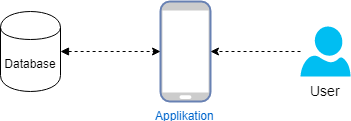
\includegraphics[height=3cm, width=8cm]{../ArkitekturDesign/OverordnetArkitektur//Oversigtoversystem}
	\caption{Oversigt over systemet.}
	\label{fig:OversigtSystembeskrivelse}
\end{figure}
Det ses på Figur \ref{fig:OversigtSystembeskrivelse}, at brugeren benytter applikationen. Applikationen kommunikerer via internettet til databasen. \\
Yderligere beskrivelse af systemet kan findes i Kravspecifikationens Afsnit \ref{Krav-sec:Systembeskrivelse} Systembeskrivelse, som er vedlagt i bilag.

\clearpage

\section{Domænemodel}
Denne domænemodel giver et overblik over, hvordan systemet er bygget op. Domæne modellen viser forbindelserne mellem de forskellige elementer i systemet og hvordan de interagerer med hinanden. Dette gør det lettere at gå fra domænemodellen til implementationen.
I dette projekt er der udarbejdet én domænemodel, som ses på Figur \ref{fig:Domain}.

\begin{figure}[H] % (alternativt [H])
	\centering
	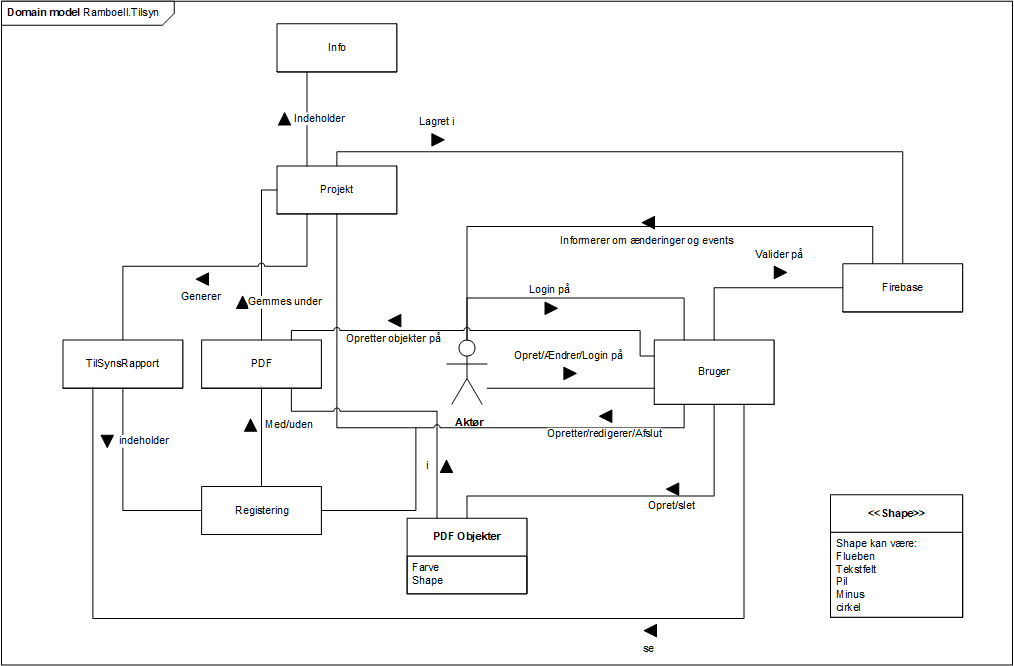
\includegraphics[height=13cm, width=17cm]{../ArkitekturDesign/OverordnetArkitektur/Domainmodel}
	\caption{Domænemodel for Rambøll Tilsyn.}
	\label{fig:Domain}
\end{figure}
Brugeren logger ind på Rambøll Tilsyn. Her kan brugeren oprette et projekt, som kan indeholde flere registreringer. I registreringen kan der tilknyttes en PDF tegning, hvorpå brugeren kan oprette forskellige objekter eller fjerne forkerte objekter. \\
Når brugeren er færdig med en registrering, vil objekter, PDF-tegning mv. blive gemt i Firebase databasen.

\clearpage

\section{Klasse diagram}
På Figur \ref{fig:KlasseDiagram} ses der en klasse diagram over Rambøll TilSyn vist i standard UML notation\cite{UML}. Klassediagrammet udpeger essentielle funktioner og felter for klassen i applikationen og visuelt viser deres relationer til hinanden.

\begin{figure}[H] % (alternativt [H])
	\centering
	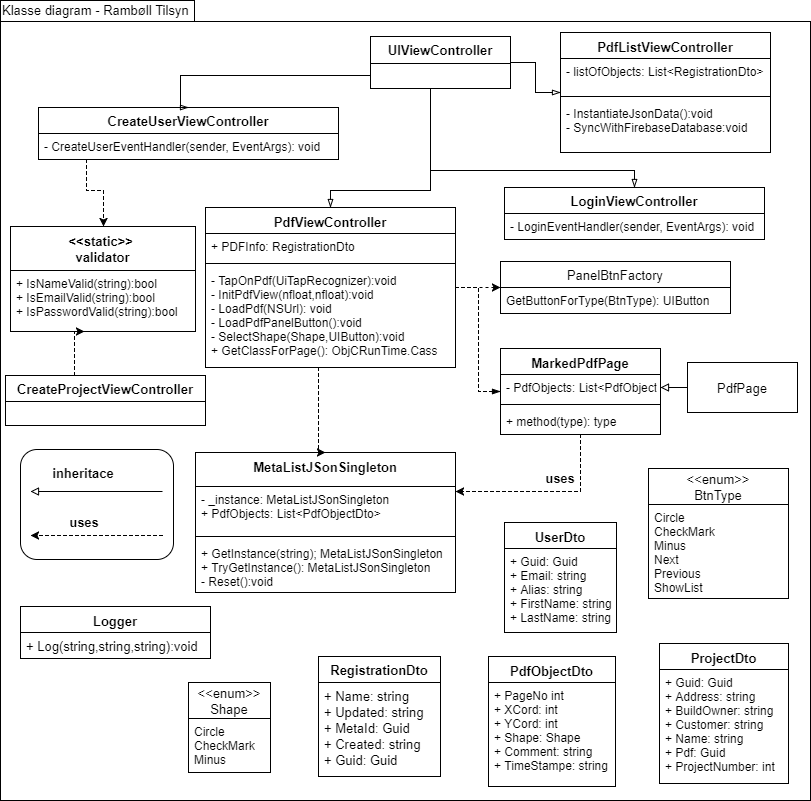
\includegraphics[height=13cm, width=17cm]{../ArkitekturDesign/OverordnetArkitektur/KlasseDiagram}
	\caption{Klassediagram for Rambøll Tilsyn.}
	\label{fig:KlasseDiagram}
\end{figure}

Her ses, at alle ViewControllers er nedarvet fra UIViewController\cite{UIViewController}, som er en klasse, der stammer fra Xamarin.iOS frameworket. UITableViewController er en specialiseret klasse fra Xamarin.iOS frameworket, der er nedarvet fra UIViewController. Formålet med denne er at vise en liste af data, som man selv har implementeret. Logger klassen bruger Firebase Analytics\cite{FirebaseAnalytic} for at logge events fra applikationen, som en erstatning for at skrive sine fejlbeskeder ud i Console lokalt\cite{CON}. Fordelen ved dette er, at man kan logge diverse events fra alle devices og se det på Firebase Console.  
